% !Mode:: "TeX:UTF-8"
\documentclass[11pt]{article}
\usepackage[letterpaper, margin = 2cm]{geometry}
\usepackage{microtype}
\usepackage{parskip}
\usepackage{amssymb}
\usepackage{amsmath}
\usepackage{multicol}
\usepackage{graphicx}
\usepackage{subcaption}
\usepackage{siunitx}
\usepackage{float}
\usepackage[style=ieee]{biblatex}
\usepackage[bookmarks, unicode]{hyperref}

\graphicspath{{helical_images/}}

\title{Regen Calculations --- Helical Channels}
\author{Josh Kraan}
\date{\today}

\begin{document}

\maketitle

\section{Purpose}

This document records the additional work done to model helical channels using the previously developed regenerative cooling model.

\section{Introduction}

Previous work showed that an annular regenerative cooling design would likely perform poorly for our use. ANSYS simulations and analyses done with Rocket Propulsion Analysis (RPA) agreed with this, so another method of regenerative cooling was required. An alternative that can be manufactured similarly to a coaxial jacket is to use a helical spacer in a coaxial jacket to produce helical cooling channels, such as was done in the LR-101 engine.

Feynman output 11 was used for the calculations in this document. A notable difference with this output was that the allowable channel pressure drop was raised to 50\% of the chamber pressure from the previous 20\%. This document will only focus on regenerative cooling of the chamber section of the engine.

\section{Helical Calculations}

Most of the previously documented work was reused. The flow was modeled similarly to the annular case, except that the hydraulic diameter and flow area were calculated from the channel height and the axial pitch of the helix. As no information could be found on modeling this type of high aspect ratio helical channel, this analysis method assumes that the helix angle is low enough and the chamber diameter is high enough that helical flow effects are negligible. The option to use multiple helixes was also included.

One change made to the method for both annular and helical channels was to calculate the fuel properties at the exit pressure of the channel, rather than the inlet. The fuel boiling point increases as pressure increases, so this distinction becomes important when the pressure drop in the cooling channels is high. Ideally, the properties should be tabulated for pressure and temperature but this would be difficult and time consuming to implement with the available REFPROP software version.

1-dimensional calculations showed that a helical channel design with a pressure drop of 50\% of the chamber pressure could take up to 64\% of the calculated heat flux before fuel boiling would begin to occur. \SI{2}{\milli\meter} and \SI{3}{\milli\meter} channel heights with spacer axial pitches of \SI{11.9}{\centi\meter} and \SI{7.6}{\centi\meter} respectively performed similarly, however the \SI{3}{\milli\meter} option has a lower pitch which would likely reduce helical flow effects, and so would likely perform better. Temperatures for the \SI{3}{\milli\meter} design are shown in Figure~\ref{fig:one_dimensional}. The high temperature at the entrance is similar to what was observed and explained for pure coaxial flow in the previous document.

\begin{figure}[H]
	\centering
  	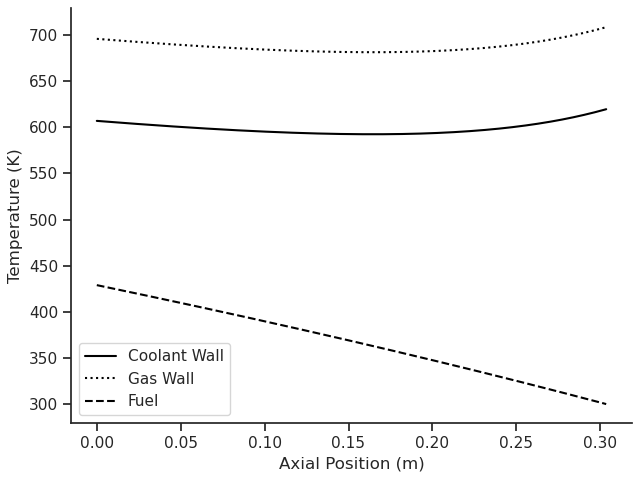
\includegraphics[width=0.7\linewidth]{Temperatures_3mm}
  	\caption{1-Dimensional Simulation Results --- \SI{3}{\milli\meter} x \SI{7.6}{\centi\meter} channel.}
  	\label{fig:one_dimensional}
\end{figure}

\section{ANSYS Simulations}

Analysis with ANSYS Fluent was conducted to double-check 1-dimensional calculations and to look at helical flow effects. Half of a helical channel was used for these calculations, as can be seen in Figure~\ref{fig:ansys_geom}. Zero heat flux boundary conditions were assumed on the outer wall and the cut surface of the spacers; if helical flow effects are significant this technically would not be correct, but as the spacer is thin and is made up of steel which has low thermal conductivity, it is predicted that this would not have a significant effect. Fuel properties were tabulated using REFPROP and processed with a Python script into a Fluent user defined material file with piecewise-linear fits.

\begin{figure}[H]
	\centering
  	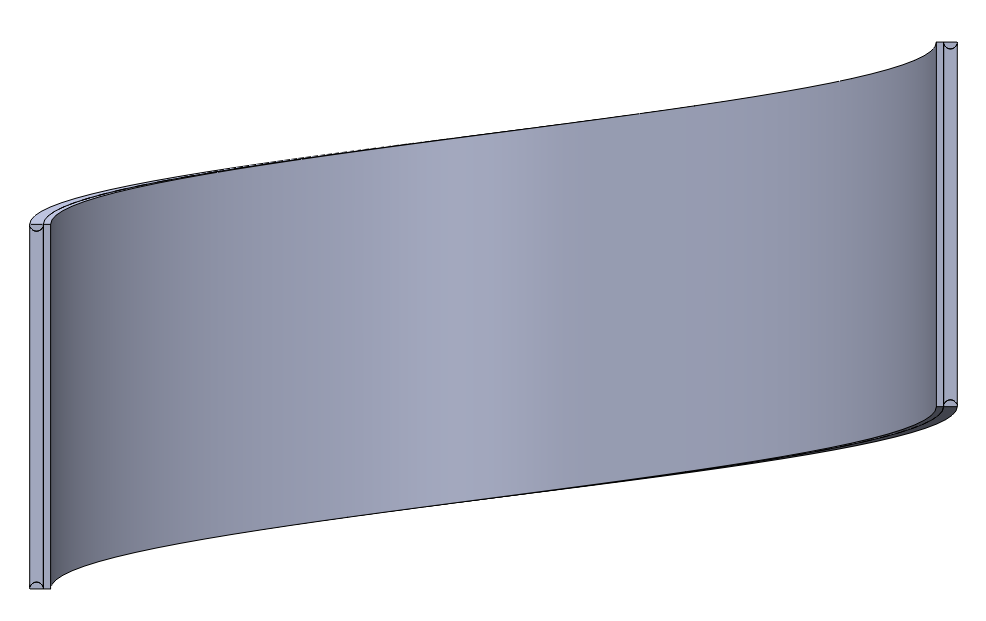
\includegraphics[width=0.6\linewidth]{solidwork_screenshot}
  	\caption{ANSYS simulation geometry.}
  	\label{fig:ansys_geom}
\end{figure}

One important detail that was neglected in the 1-dimensional simulation but is included in the ANSYS simulation is the effect of the spacer. The spacer slightly reduces the flow area, and slows the fluids in gaps near it, potentially leading to hot spots.

For this comparison between ANSYS and the 1-dimensional simulation, a \SI{3}{\milli\meter} channel with an axial pitch of \SI{8}{\centi\meter} and a heat flux of 60\% of predicted was used.

Entrance effects were found to be significant, as can be seen in Figure~\ref{fig:entrance}, but disappeared about halfway through the channel length. Helical flow effects are also clearly visible in Figure~\ref{fig:helical}. While 1-dimensional calculations predict a flow velocity of approximately \SI{10}{\meter\per\second}, in the ANSYS simulation one side has a velocity of \SI{7}{\meter\per\second} and the other \SI{14}{\meter\per\second}.

\begin{figure}[H]
	\centering
	\begin{subfigure}{.5\textwidth}
		\centering
		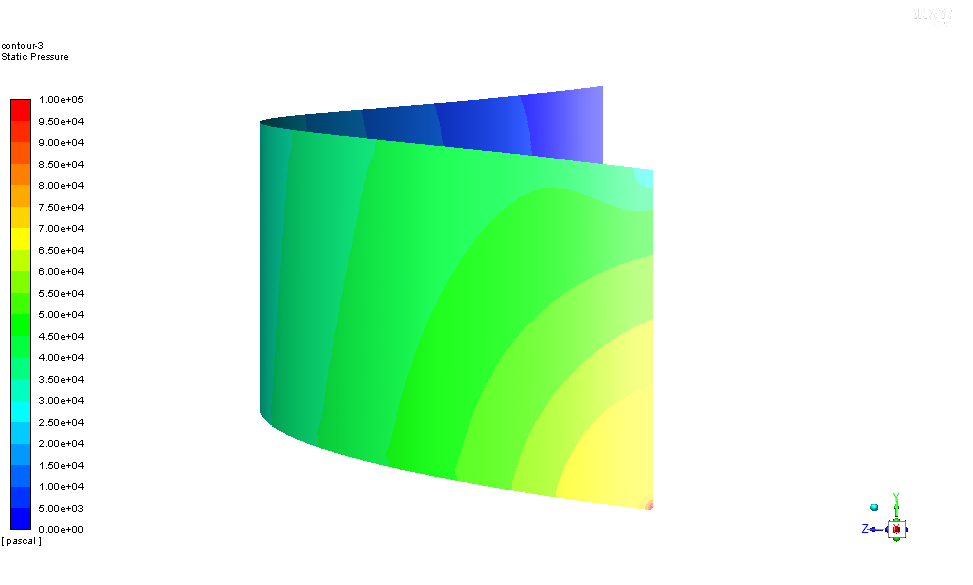
\includegraphics[width=.9\linewidth, trim={0 0 5cm 0}, clip]{pressure-1}
		\caption{Pressure.}
	\end{subfigure}%
	\begin{subfigure}{.5\textwidth}
		\centering
  		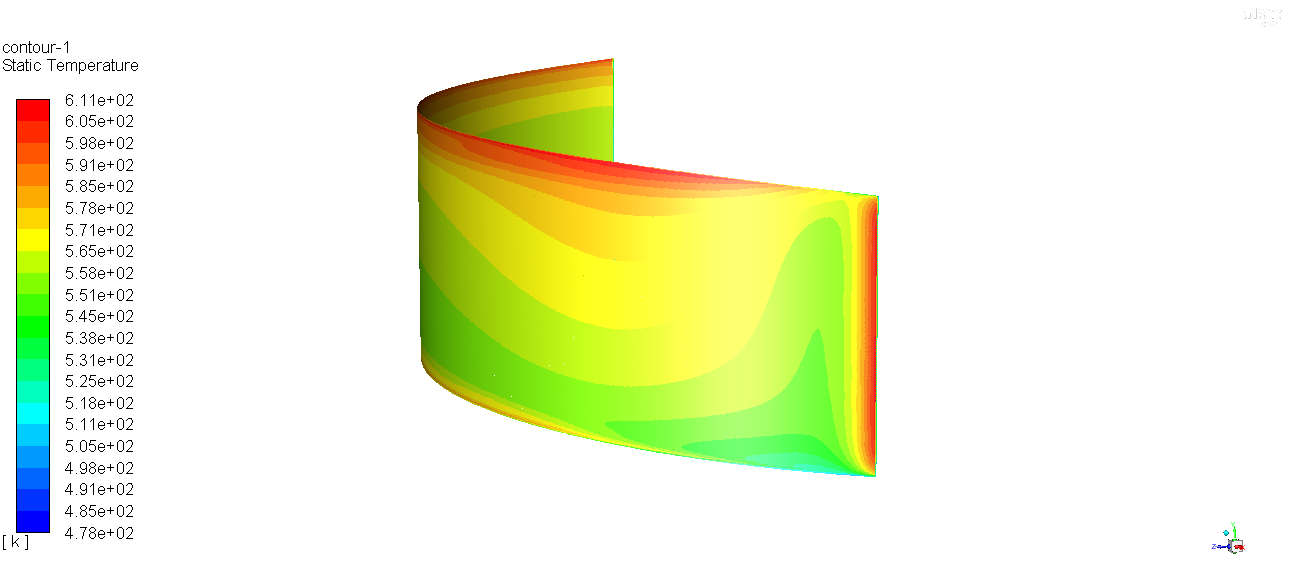
\includegraphics[width=.9\linewidth, trim={0 0 12cm 0}, clip]{temperature-2}
  		\caption{Temperature.}
	\end{subfigure}
	\caption{Entrance effects.}
	\label{fig:entrance}
\end{figure}

\begin{figure}[H]
	\centering
	\begin{subfigure}{.7\textwidth}
		\centering
		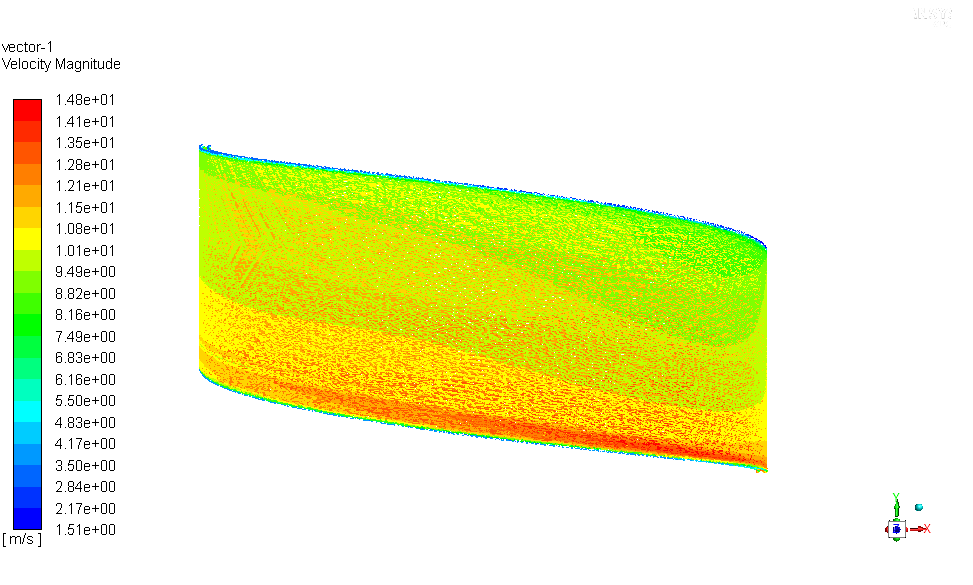
\includegraphics[width=0.9\linewidth, trim={0 0 5cm 0}, clip]{velocity}
		\caption{Channel.}
	\end{subfigure}%
	\begin{subfigure}{.3\textwidth}
		\centering
  		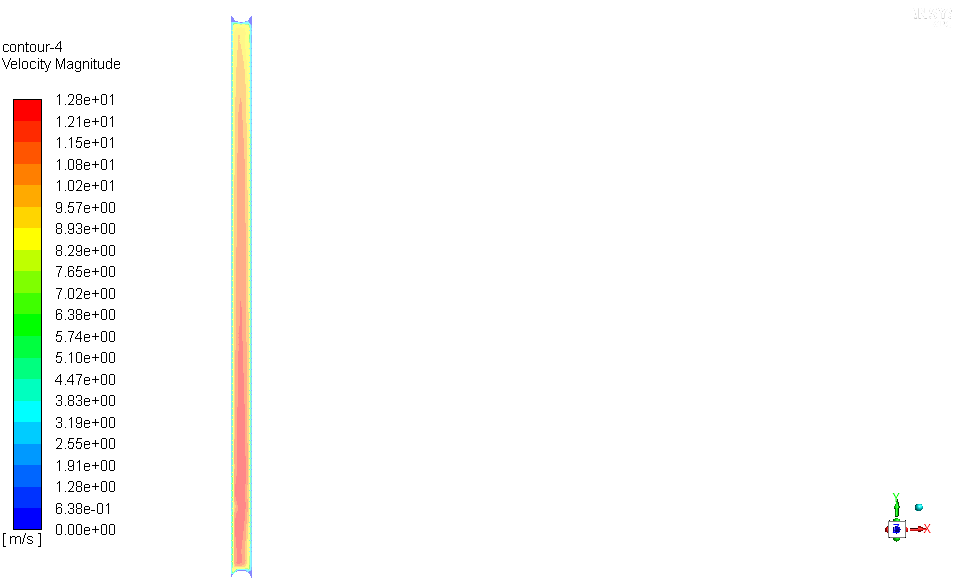
\includegraphics[width=0.9\linewidth, trim={0 0 20cm 0}, clip]{velocitiy-2}
  		\caption{Cross section.}
	\end{subfigure}
	\caption{Helical flow effects.}
	\label{fig:helical}
\end{figure}

The pressure drop for the entire cooling channel was estimated from this section. Pressure contours in this channel section can be seen in Figure~\ref{fig:pressure_contours}. The pressure difference between halfway through this section and the exit was found to be approximately \SI{28}{\kilo\pascal}. When scaled to the entire chamber cooling channel, this gives a pressure drop of \SI{425}{\kilo\pascal} --- a 1\% difference from the \SI{429}{\kilo\pascal} predicted by the 1-dimensional calculations.

\begin{figure}[H]
	\centering
  	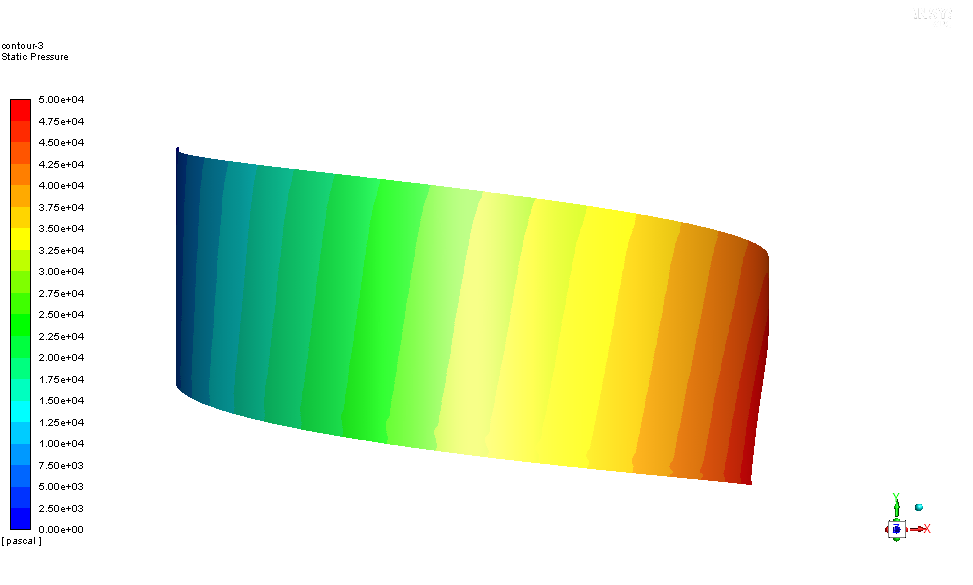
\includegraphics[width=0.7\linewidth, trim={0 0 5cm 0}, clip]{pressure-2}
  	\caption{Channel pressure contours.}
  	\label{fig:pressure_contours}
\end{figure}

To compare the ANSYS results to the 1-dimensional calculations, 3 ANSYS simulations were run with different inlet fuel temperatures corresponding to different locations along the chamber. Temperature contours near the exit for an inlet temperature of \SI{411}{\kelvin} are shown in Figure~\ref{fig:temp_contours}, and a comparison between ANSYS and the 1-dimensional calculations is shown in Figure~\ref{fig:comparison}.

\begin{figure}[H]
	\centering
  	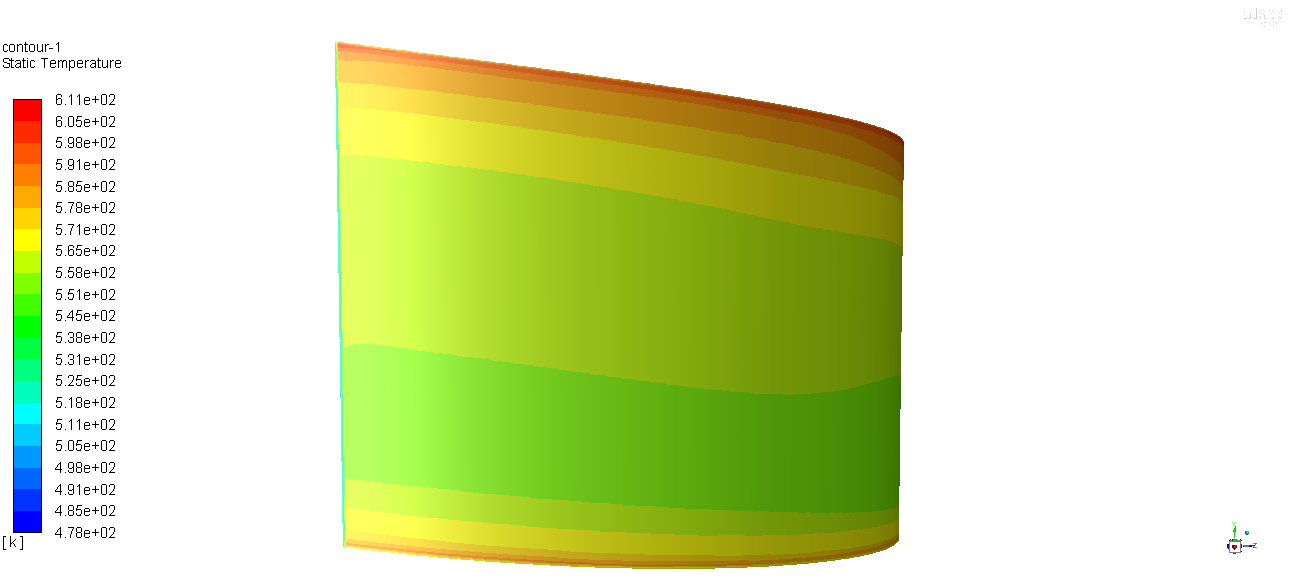
\includegraphics[width=0.7\linewidth, trim={0 0 5cm 0}, clip]{temperature-3}
  	\caption{Channel temperature contours.}
  	\label{fig:temp_contours}
\end{figure}

\begin{figure}[H]
	\centering
  	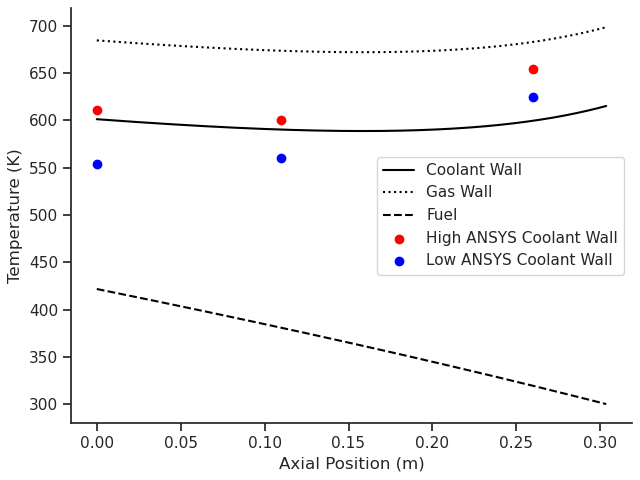
\includegraphics[width=0.7\linewidth]{Temperatures_ANSYS}
  	\caption{ANSYS and 1-dimensional simulation comparison.}
  	\label{fig:comparison}
\end{figure}

The highest coolant wall temperatures calculated by ANSYS for the 2 locations closest to the injector are quite close to the 1-dimensional calculations. This could be because of reduced flow area (and decreased temperature) due to to the spacer volume combined with increased temperature due to the local flow restriction of the spacer gap.

The point closest to the coolant inlet is significantly higher than what was calculated. As the temperature is beyond the boiling point of the fluid, it was produced by extrapolating the tabulated fluid properties. This means this result cannot be trusted, however it could indicate inaccuracies in the model which physical testing may pinpoint.

\section{Inner Wall Temperature Limits}

Simulations so far have focused on the inner wall temperature where boiling occurs as a limit, but it is quite likely that buckling of the inner wall would put a limit on the temperature that it can handle. As the system encounters higher heat fluxes the temperature gradient in the wall will increase, at some point it will likely become limiting.

A thermal conductivity of \SI{50}{\watt\per\meter\per\kelvin} has been used for these calculations, which seems to be close to the upper range of thermal conductivities for typical steels. Reducing this thermal conductivity would significantly increase the gas wall temperature.

\section{Conclusion}

The helical channel design was shown to be theoretically capable of handling much higher heat fluxes than coaxial shells (64\% vs 19\%) but it has an enormously higher pressure drop (50\% vs 4\%).

Even when using the entire allotted channel pressure drop for the chamber alone, film cooling would be required to keep the fuel from boiling. Additionally, at higher heat fluxes the steel wall would likely have to be replaced with a higher thermal conductivity material such as copper.

It seems likely that regenerative cooling will not be possible unless the heat flux is much lower than predicted, film cooling performs very well, or some kind of thermal barrier coating is applied to the engine walls.


\end{document}
